\begin{itemize}
    \item Question type distribution. We curate most frequently occurring top 200 bi-gram and tri-gram patterns and partition them into different categories based on domain knowledge. For example, the patterns with words ``longest", ``shortest"", and farthest etc. would require sorting.
   This heuristic-based approximate question distribution is shown in \figref{answer_distrib}
    \item types of reasoning needed to answer questions \tabref{interesting_example}
    \item distribution of answer types - span, number, digit
    \item What's \emph{not} in the data: common sense inference, except for lexical relationships (e.g., grandfather $==$ mother's father).  Some questions require knowledge of scoring in sports; there are enough examples of these that the model at least has a chance of learning this from the data.
\end{itemize}

\begin{figure}
    \centering
    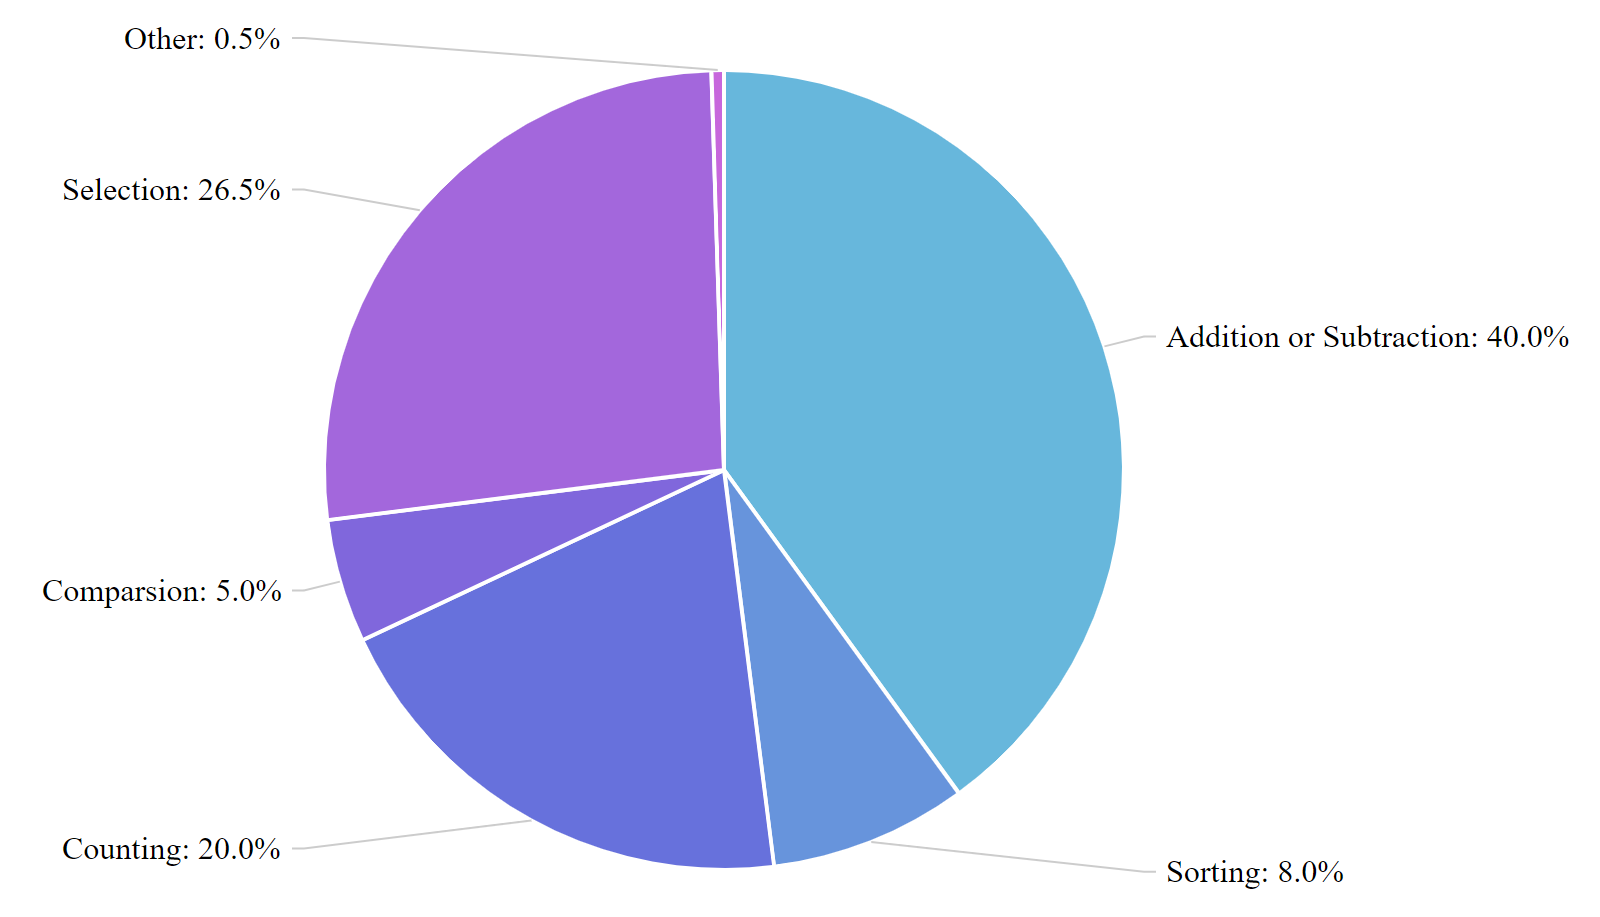
\includegraphics[width=0.5\textwidth]{images/answer_distrib}
    \caption{Distribution of categories of questions}
    \label{fig:answer_distrib}
\end{figure}
\gabi{Consider removing this figure 
and putting numbers in Table 1}

\begin{table*}[t]
\centering
\footnotesize
\begin{tabular}{|p{1.5cm}|p{8cm}|p{3cm}|p{1.25cm}|p{1.25cm}|}
\hline
Reasoning & Passage & Question & Answer & BiDAF Answer\\
 \hline
 Addition or Subtraction & Before the UNPROFOR fully deployed, the HV clashed with an armed force of the RSK in the village of Nos Kalik, located in a pink zone near \u Sibenik, and captured the village at 4:45p.m. on {\color{teal}2 March 1992}. The JNA formed a battlegroup to counterattack the {\color{teal}next day}. & What date did the JNA form a battlegroup to counterattack after the village of Nos Kalik was captured?  & 3 March 1992 & 2 March 1992 \\ 
 \hline
 Comparison & In {\color{orange}1517, the seventeen-year-old King sailed to Castile}, where he was formally recognised as King of Castile. There, his Flemish court provoked much scandal, as de Cro\"y shamelessly sold government privileges for personal money and installed other Flemish nobles into government offices. {\color{orange}In May 1518, Charles traveled to Barcelona in Aragon}, where he would remain for nearly two years. & Where did Charles travel to first, Castile or Barcelona? & Castile & Aragon\\
 \hline
 Selection & In 1970, to commemorate the 100th anniversary of the founding of Baldwin City, {\color{purple}Baker University professor and playwright Don Mueller and Phyllis E. Braun, Business Manager, produced a musical play entitled The Ballad Of Black Jack} to tell the story of the events that led up to the battle. & Who was the University professor that helped produce The Ballad Of Black Jack, Ivan Boyd or Don Mueller? & Don Mueller & Baker\\
 \hline
 Count and Sort & Denver would retake the lead with kicker {\color{brown}Matt Prater nailing a 43-yard field goal}, yet Carolina answered as kicker {\color{brown}John Kasay ties the game with a 39-yard field goal}. In the second quarter, Carolina took the lead with rookie RB Jonathan Stewart getting a 2-yard TD run. Carolina closed out the half with {\color{brown}Kasay nailing a 44-yard field goal}. In the third quarter, Carolina increased its lead with RB DeAngelo Williams's 56-yard TD run for the only score of the period. In the fourth quarter, Carolina sealed the win with {\color{brown}Kasay's 42-yard field goal}. & Which kicker kicked the most field goals? & John Kasay & Matt Prater\\
 \hline
 Set of spans & Charleston is a popular tourist destination, {\color{teal}with a considerable number of hotels, inns, and bed and breakfasts}, numerous restaurants featuring Lowcountry cuisine and shops. Charleston is also a notable art destination, named a top-25 arts destination by AmericanStyle magazine. & What type of accommodations are available in Charleston? &``hotels", ``inns", ``bed and breakfasts" & top-25 arts\\
 \hline
 Complex Composition & James Douglas was the second {\color{olive}son of Sir George Douglas of Pittendreich, Master of Angus, and Elizabeth Douglas, daughter of David Douglas} of Pittendreich & Who was the grandfather of James Douglas? & David Douglas & Sir George Douglas\\
 \hline
 Complex entity and coreference Resolution & {\color{violet}James Douglas} was the second son of Sir George Douglas of Pittendreich, Master of Angus, and Elizabeth Douglas, daughter David Douglas of Pittendreich. He wrote that he was over 61 years old in March 1578, so was probably born around 1516. Before {\color{violet}1543 he married Elizabeth}, daughter of James Douglas, 3rd Earl of Morton. {\color{violet}In 1553 James Douglas succeeded to the title and estates of his father-in-law}, including Dalkeith House in Midlothian, and Aberdour Castle in Fife. & How many years after he married Elizabeth did James Douglas succeed to the title and estates of his father-in-law? & 10 & 1553\\
 \hline
 
\end{tabular}
\caption{Different reasoning required to answer questions in the dataset}
\label{tab:interesting_example}
\end{table*}

\gabi{Make sure that the Table 1 fits the paper, consider moving to the second page, also maybe add SOTA's answer, and not neccessarily BIDAF's}